\chapter{Алгоритм решения}
Обозначим через $f_{\mathrm{A}}$ и $f*$ приближенное (полученное при помощи алгоритма $\mathrm{A}$) 
и оптимальное значение целевой функции функции в некоторой конкретной задаче соответсвенно.

Будем говорить, что алгоритм  $\mathrm{A}$ имеет оценки $(\epsilon_{\mathrm{A}}, \delta_{\mathrm{A}})$
если выполнено неравентво 
\[
Pr \{ f_{\mathrm{A}} > (1+ \epsilon_{\mathrm{A}} f* \} \leq \delta_{\mathrm{A}}
\],
где $\epsilon_{\mathrm{A}}$ есть оценка относительной погрешности решния, получаемого алгоритмом ${\mathrm{A}}$,
$\delta_{\mathrm{A}}$ -- вероятность несрабатывания алгоритма ${\mathrm{A}}$, что можно трактовать как долю случаев, когда алгоритм А не гарантирует точность в пределах $\epsilon_{\mathrm{A}}$.

Алгоритм А назвается асимптотически оптимальным если существую оценки $(\epsilon_{\mathrm{A}}, \delta_{\mathrm{A}})$
стремящиеся к нулю с ростом размерности. 

\section{Алгоритм}
Через $\phi$ обозначим любую целочислено значащую функцию, при этом $1 < \phi_n < n$ 
\begin{enumerate}
\item Берем произвольную подстановку $\pi \in S_n$. Пусть $(d_{jk})$ - $n \times n$ 
матрица, содержащая элементы исходной матрицы $(c_{ijk})$, где индекс $j=\pi(i)$ такой, что
$$
d_{ij} = c_{\pi^{-1}(j)jk}
$$
для любых $1 \leq j$,$n \leq n$
Положим $f = 0 ; j =1 ; \mathrm{K}={1,2, \ldots , \phi_n}$. 
\item Выберем номер $\sigma(j)$ минимального элемента из множества $\mathrm{argmin} \, {d_{jk} | k \in K}$.
\item Полагаем $f = f + d_{j \sigma (j)} ; \mathrm{K} = \mathrm{K}  \setminus  {\sigma(j)} ; k=j+\phi_n$
\item Если $k \leq n $, то $K = K \bigcap {k}$.
\item $j = j + 1$
\item Повторяем п.2, пока j<n. В противном случае идем к п.7
\item Результатом работы алгоритма $\mathrm{A}(\phi_n)$ является значение функции $f$ целевой функции   
$f_{\mathrm{A}(\phi_n)}$. 
\end{enumerate}
\section{Блок-схема}

\begin{figure}[hp!]
  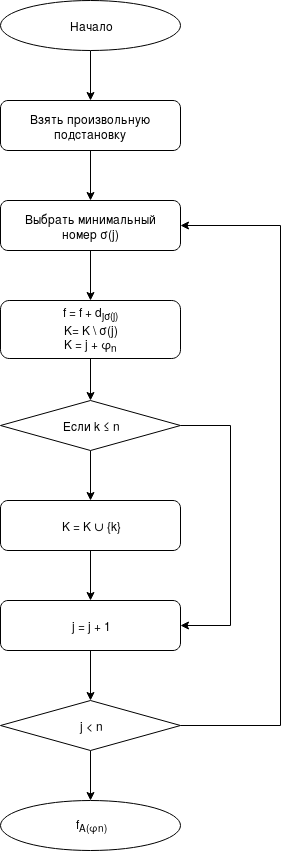
\includegraphics[width=\linewidth, height=\textheight,keepaspectratio]{Chapters/image/flowchart.png}
  \caption{A boat.}
  \label{fig:flowchart}
\end{figure}

\section{Комментарии к алгоритму}
Асимптотическое поведение трехиндексной аксиальной задачи о назначениях значительно отличается от поведения 
классической задачи о назначениях. В ряде статей Grundel Krohmal Oleveira было изучено поведение ожидаемого значения  оптимальной функции. 
Ими было доказано, что оно стремится к левой границе распределения весовых коэфициентов.

Лемма

Алгоритм А находит решение 3-АЗН за время $O(n \phi_n)$

Несмотря на то, что алгоритм показывает полиномиальное время выполения, возможен ряд улучшений
Например, заметно что алгоритм неустойчив относительно выбора начальной перестановки
\section{Вводимые модификации}
\subsection{Генерация нескольких начальных перестановок}
Изменим алгортим следующим образом

Пусть на начальном этапе дается не одна случайная перестановка, 
а $m$. Тогда на выходе можем выбрать лучшую ... Бред
\subsection{Выбор лучшей перестановки}
Введем функционал вида 

При известном точном решении будем говорить, что одна перестановка лучше другой
если она за тоже число шагов будет ближе сходится к точному решению 


\section{Итеративный алгоритм}
Добавим следующие шаги
После последнего шага сохраним результат, пойдем в начало и запустим алгоритм еще раз
Повторим M раз
Получим М выводов, в качестве ответа выберем устредненное значение. 